\documentclass[1p]{elsarticle_modified}
%\bibliographystyle{elsarticle-num}

%\usepackage[colorlinks]{hyperref}
%\usepackage{abbrmath_seonhwa} %\Abb, \Ascr, \Acal ,\Abf, \Afrak
\usepackage{amsfonts}
\usepackage{amssymb}
\usepackage{amsmath}
\usepackage{amsthm}
\usepackage{scalefnt}
\usepackage{amsbsy}
\usepackage{kotex}
\usepackage{caption}
\usepackage{subfig}
\usepackage{color}
\usepackage{graphicx}
\usepackage{xcolor} %% white, black, red, green, blue, cyan, magenta, yellow
\usepackage{float}
\usepackage{setspace}
\usepackage{hyperref}

\usepackage{tikz}
\usetikzlibrary{arrows}

\usepackage{multirow}
\usepackage{array} % fixed length table
\usepackage{hhline}

%%%%%%%%%%%%%%%%%%%%%
\makeatletter
\renewcommand*\env@matrix[1][\arraystretch]{%
	\edef\arraystretch{#1}%
	\hskip -\arraycolsep
	\let\@ifnextchar\new@ifnextchar
	\array{*\c@MaxMatrixCols c}}
\makeatother %https://tex.stackexchange.com/questions/14071/how-can-i-increase-the-line-spacing-in-a-matrix
%%%%%%%%%%%%%%%

\usepackage[normalem]{ulem}

\newcommand{\msout}[1]{\ifmmode\text{\sout{\ensuremath{#1}}}\else\sout{#1}\fi}
%SOURCE: \msout is \stkout macro in https://tex.stackexchange.com/questions/20609/strikeout-in-math-mode

\newcommand{\cancel}[1]{
	\ifmmode
	{\color{red}\msout{#1}}
	\else
	{\color{red}\sout{#1}}
	\fi
}

\newcommand{\add}[1]{
	{\color{blue}\uwave{#1}}
}

\newcommand{\replace}[2]{
	\ifmmode
	{\color{red}\msout{#1}}{\color{blue}\uwave{#2}}
	\else
	{\color{red}\sout{#1}}{\color{blue}\uwave{#2}}
	\fi
}

\newcommand{\Sol}{\mathcal{S}} %segment
\newcommand{\D}{D} %diagram
\newcommand{\A}{\mathcal{A}} %arc


%%%%%%%%%%%%%%%%%%%%%%%%%%%%%5 test

\def\sl{\operatorname{\textup{SL}}(2,\Cbb)}
\def\psl{\operatorname{\textup{PSL}}(2,\Cbb)}
\def\quan{\mkern 1mu \triangleright \mkern 1mu}

\theoremstyle{definition}
\newtheorem{thm}{Theorem}[section]
\newtheorem{prop}[thm]{Proposition}
\newtheorem{lem}[thm]{Lemma}
\newtheorem{ques}[thm]{Question}
\newtheorem{cor}[thm]{Corollary}
\newtheorem{defn}[thm]{Definition}
\newtheorem{exam}[thm]{Example}
\newtheorem{rmk}[thm]{Remark}
\newtheorem{alg}[thm]{Algorithm}

\newcommand{\I}{\sqrt{-1}}
\begin{document}

%\begin{frontmatter}
%
%\title{Boundary parabolic representations of knots up to 8 crossings}
%
%%% Group authors per affiliation:
%\author{Yunhi Cho} 
%\address{Department of Mathematics, University of Seoul, Seoul, Korea}
%\ead{yhcho@uos.ac.kr}
%
%
%\author{Seonhwa Kim} %\fnref{s_kim}}
%\address{Center for Geometry and Physics, Institute for Basic Science, Pohang, 37673, Korea}
%\ead{ryeona17@ibs.re.kr}
%
%\author{Hyuk Kim}
%\address{Department of Mathematical Sciences, Seoul National University, Seoul 08826, Korea}
%\ead{hyukkim@snu.ac.kr}
%
%\author{Seokbeom Yoon}
%\address{Department of Mathematical Sciences, Seoul National University, Seoul, 08826,  Korea}
%\ead{sbyoon15@snu.ac.kr}
%
%\begin{abstract}
%We find all boundary parabolic representation of knots up to 8 crossings.
%
%\end{abstract}
%\begin{keyword}
%    \MSC[2010] 57M25 
%\end{keyword}
%
%\end{frontmatter}

%\linenumbers
%\tableofcontents
%
\newcommand\colored[1]{\textcolor{white}{\rule[-0.35ex]{0.8em}{1.4ex}}\kern-0.8em\color{red} #1}%
%\newcommand\colored[1]{\textcolor{white}{ #1}\kern-2.17ex	\textcolor{white}{ #1}\kern-1.81ex	\textcolor{white}{ #1}\kern-2.15ex\color{red}#1	}

{\Large $\underline{12a_{0445}~(K12a_{0445})}$}

\setlength{\tabcolsep}{10pt}
\renewcommand{\arraystretch}{1.6}
\vspace{1cm}\begin{tabular}{m{100pt}>{\centering\arraybackslash}m{274pt}}
\multirow{5}{120pt}{
	\centering
	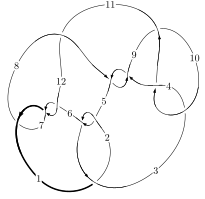
\includegraphics[width=112pt]{../../../GIT/diagram.site/Diagrams/png/1246_12a_0445.png}\\
\ \ \ A knot diagram\footnotemark}&
\allowdisplaybreaks
\textbf{Linearized knot diagam} \\
\cline{2-2}
 &
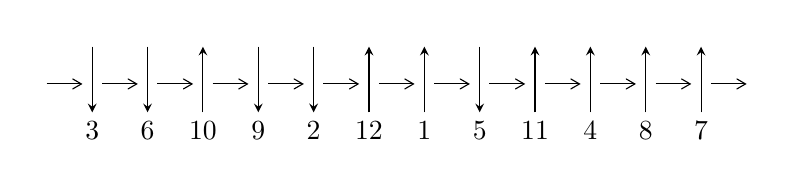
\begin{tikzpicture}[x=20pt, y=17pt]
	% nodes
	\node (C0) at (0, 0) {};
	\node (C1) at (1, 0) {};
	\node (C1U) at (1, +1) {};
	\node (C1D) at (1, -1) {3};

	\node (C2) at (2, 0) {};
	\node (C2U) at (2, +1) {};
	\node (C2D) at (2, -1) {6};

	\node (C3) at (3, 0) {};
	\node (C3U) at (3, +1) {};
	\node (C3D) at (3, -1) {10};

	\node (C4) at (4, 0) {};
	\node (C4U) at (4, +1) {};
	\node (C4D) at (4, -1) {9};

	\node (C5) at (5, 0) {};
	\node (C5U) at (5, +1) {};
	\node (C5D) at (5, -1) {2};

	\node (C6) at (6, 0) {};
	\node (C6U) at (6, +1) {};
	\node (C6D) at (6, -1) {12};

	\node (C7) at (7, 0) {};
	\node (C7U) at (7, +1) {};
	\node (C7D) at (7, -1) {1};

	\node (C8) at (8, 0) {};
	\node (C8U) at (8, +1) {};
	\node (C8D) at (8, -1) {5};

	\node (C9) at (9, 0) {};
	\node (C9U) at (9, +1) {};
	\node (C9D) at (9, -1) {11};

	\node (C10) at (10, 0) {};
	\node (C10U) at (10, +1) {};
	\node (C10D) at (10, -1) {4};

	\node (C11) at (11, 0) {};
	\node (C11U) at (11, +1) {};
	\node (C11D) at (11, -1) {8};

	\node (C12) at (12, 0) {};
	\node (C12U) at (12, +1) {};
	\node (C12D) at (12, -1) {7};
	\node (C13) at (13, 0) {};

	% arrows
	\draw[->,>={angle 60}]
	(C0) edge (C1) (C1) edge (C2) (C2) edge (C3) (C3) edge (C4) (C4) edge (C5) (C5) edge (C6) (C6) edge (C7) (C7) edge (C8) (C8) edge (C9) (C9) edge (C10) (C10) edge (C11) (C11) edge (C12) (C12) edge (C13) ;	\draw[->,>=stealth]
	(C1U) edge (C1D) (C2U) edge (C2D) (C3D) edge (C3U) (C4U) edge (C4D) (C5U) edge (C5D) (C6D) edge (C6U) (C7D) edge (C7U) (C8U) edge (C8D) (C9D) edge (C9U) (C10D) edge (C10U) (C11D) edge (C11U) (C12D) edge (C12U) ;
	\end{tikzpicture} \\
\hhline{~~} \\& 
\textbf{Solving Sequence} \\ \cline{2-2} 
 &
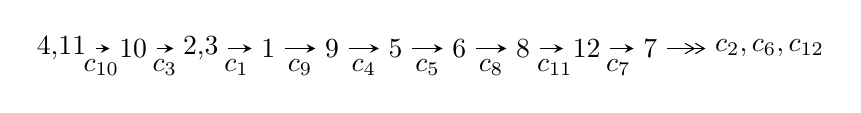
\begin{tikzpicture}[x=23pt, y=7pt]
	% node
	\node (A0) at (-1/8, 0) {4,11};
	\node (A1) at (1, 0) {10};
	\node (A2) at (33/16, 0) {2,3};
	\node (A3) at (25/8, 0) {1};
	\node (A4) at (33/8, 0) {9};
	\node (A5) at (41/8, 0) {5};
	\node (A6) at (49/8, 0) {6};
	\node (A7) at (57/8, 0) {8};
	\node (A8) at (65/8, 0) {12};
	\node (A9) at (73/8, 0) {7};
	\node (C1) at (1/2, -1) {$c_{10}$};
	\node (C2) at (3/2, -1) {$c_{3}$};
	\node (C3) at (21/8, -1) {$c_{1}$};
	\node (C4) at (29/8, -1) {$c_{9}$};
	\node (C5) at (37/8, -1) {$c_{4}$};
	\node (C6) at (45/8, -1) {$c_{5}$};
	\node (C7) at (53/8, -1) {$c_{8}$};
	\node (C8) at (61/8, -1) {$c_{11}$};
	\node (C9) at (69/8, -1) {$c_{7}$};
	\node (A10) at (11, 0) {$c_{2},c_{6},c_{12}$};

	% edge
	\draw[->,>=stealth]	
	(A0) edge (A1) (A1) edge (A2) (A2) edge (A3) (A3) edge (A4) (A4) edge (A5) (A5) edge (A6) (A6) edge (A7) (A7) edge (A8) (A8) edge (A9) ;
	\draw[->>,>={angle 60}]	
	(A9) edge (A10);
\end{tikzpicture} \\ 

\end{tabular} \\

\footnotetext{
The image of knot diagram is generated by the software ``\textbf{Draw programme}" developed by Andrew Bartholomew(\url{http://www.layer8.co.uk/maths/draw/index.htm\#Running-draw}), where we modified some parts for our purpose(\url{https://github.com/CATsTAILs/LinksPainter}).
}\phantom \\ \newline 
\centering \textbf{Ideals for irreducible components\footnotemark of $X_{\text{par}}$} 
 
\begin{align*}
I^u_{1}&=\langle 
- u^{60}+16 u^{58}+\cdots+4 b+4,\;2 u^{64}-34 u^{62}+\cdots+4 a-2,\;u^{65}-2 u^{64}+\cdots+4 u-2\rangle \\
I^u_{2}&=\langle 
-7 u^8 a^2+2 u^8 a+\cdots-8 a+8,\;-3 u^8 a- u^8+\cdots- a-1,\;u^9+u^8-2 u^7-3 u^6+u^5+3 u^4+2 u^3- u-1\rangle \\
I^u_{3}&=\langle 
u^3+b- u+1,\;- u^3-2 u^2+2 a+2 u+2,\;u^4-2 u^2+2\rangle \\
\\
I^v_{1}&=\langle 
a,\;b+1,\;v-1\rangle \\
\end{align*}
\raggedright * 4 irreducible components of $\dim_{\mathbb{C}}=0$, with total 97 representations.\\
\footnotetext{All coefficients of polynomials are rational numbers. But the coefficients are sometimes approximated in decimal forms when there is not enough margin.}
\newpage
\renewcommand{\arraystretch}{1}
\centering \section*{I. $I^u_{1}= \langle - u^{60}+16 u^{58}+\cdots+4 b+4,\;2 u^{64}-34 u^{62}+\cdots+4 a-2,\;u^{65}-2 u^{64}+\cdots+4 u-2 \rangle$}
\flushleft \textbf{(i) Arc colorings}\\
\begin{tabular}{m{7pt} m{180pt} m{7pt} m{180pt} }
\flushright $a_{4}=$&$\begin{pmatrix}0\\u\end{pmatrix}$ \\
\flushright $a_{11}=$&$\begin{pmatrix}1\\0\end{pmatrix}$ \\
\flushright $a_{10}=$&$\begin{pmatrix}1\\u^2\end{pmatrix}$ \\
\flushright $a_{2}=$&$\begin{pmatrix}-\frac{1}{2} u^{64}+\frac{17}{2} u^{62}+\cdots-2 u^2+\frac{1}{2}\\\frac{1}{4} u^{60}-4 u^{58}+\cdots+\frac{3}{2} u-1\end{pmatrix}$ \\
\flushright $a_{3}=$&$\begin{pmatrix}- u\\- u^3+u\end{pmatrix}$ \\
\flushright $a_{1}=$&$\begin{pmatrix}-\frac{1}{2} u^{64}+\frac{17}{2} u^{62}+\cdots+u+\frac{1}{2}\\\frac{3}{4} u^{57}-\frac{45}{4} u^{55}+\cdots+\frac{1}{2} u-1\end{pmatrix}$ \\
\flushright $a_{9}=$&$\begin{pmatrix}- u^2+1\\u^2\end{pmatrix}$ \\
\flushright $a_{5}=$&$\begin{pmatrix}- u^5+2 u^3- u\\u^5- u^3+u\end{pmatrix}$ \\
\flushright $a_{6}=$&$\begin{pmatrix}-\frac{1}{2} u^{64}+u^{63}+\cdots-\frac{1}{2} u^2-\frac{1}{2}\\u^{64}- u^{63}+\cdots-\frac{3}{2} u+1\end{pmatrix}$ \\
\flushright $a_{8}=$&$\begin{pmatrix}- u^8+3 u^6-3 u^4+1\\u^8-2 u^6+2 u^4\end{pmatrix}$ \\
\flushright $a_{12}=$&$\begin{pmatrix}u^{16}-5 u^{14}+11 u^{12}-12 u^{10}+5 u^8+2 u^6-2 u^4+1\\- u^{16}+4 u^{14}-8 u^{12}+8 u^{10}-4 u^8\end{pmatrix}$ \\
\flushright $a_{7}=$&$\begin{pmatrix}-\frac{1}{4} u^{47}+3 u^{45}+\cdots-\frac{1}{2} u+1\\-\frac{1}{4} u^{49}+\frac{13}{4} u^{47}+\cdots+\frac{1}{2} u^2+\frac{1}{2} u\end{pmatrix}$\\&\end{tabular}
\flushleft \textbf{(ii) Obstruction class $= -1$}\\~\\
\flushleft \textbf{(iii) Cusp Shapes $= 2 u^{64}-34 u^{62}+\cdots+4 u^2+2 u$}\\~\\
\newpage\renewcommand{\arraystretch}{1}
\flushleft \textbf{(iv) u-Polynomials at the component}\newline \\
\begin{tabular}{m{50pt}|m{274pt}}
Crossings & \hspace{64pt}u-Polynomials at each crossing \\
\hline $$\begin{aligned}c_{1}\end{aligned}$$&$\begin{aligned}
&u^{65}+30 u^{64}+\cdots+341 u+25
\end{aligned}$\\
\hline $$\begin{aligned}c_{2},c_{5}\end{aligned}$$&$\begin{aligned}
&u^{65}+2 u^{64}+\cdots- u-5
\end{aligned}$\\
\hline $$\begin{aligned}c_{3},c_{10}\end{aligned}$$&$\begin{aligned}
&u^{65}-2 u^{64}+\cdots+4 u-2
\end{aligned}$\\
\hline $$\begin{aligned}c_{4},c_{8}\end{aligned}$$&$\begin{aligned}
&u^{65}-6 u^{64}+\cdots+800 u-128
\end{aligned}$\\
\hline $$\begin{aligned}c_{6},c_{7},c_{12}\end{aligned}$$&$\begin{aligned}
&u^{65}-2 u^{64}+\cdots-29 u-5
\end{aligned}$\\
\hline $$\begin{aligned}c_{9}\end{aligned}$$&$\begin{aligned}
&u^{65}-34 u^{64}+\cdots+8 u-4
\end{aligned}$\\
\hline $$\begin{aligned}c_{11}\end{aligned}$$&$\begin{aligned}
&u^{65}+6 u^{64}+\cdots-38400 u-6400
\end{aligned}$\\
\hline
\end{tabular}\\~\\
\newpage\renewcommand{\arraystretch}{1}
\flushleft \textbf{(v) Riley Polynomials at the component}\newline \\
\begin{tabular}{m{50pt}|m{274pt}}
Crossings & \hspace{64pt}Riley Polynomials at each crossing \\
\hline $$\begin{aligned}c_{1}\end{aligned}$$&$\begin{aligned}
&y^{65}+18 y^{64}+\cdots-5119 y-625
\end{aligned}$\\
\hline $$\begin{aligned}c_{2},c_{5}\end{aligned}$$&$\begin{aligned}
&y^{65}-30 y^{64}+\cdots+341 y-25
\end{aligned}$\\
\hline $$\begin{aligned}c_{3},c_{10}\end{aligned}$$&$\begin{aligned}
&y^{65}-34 y^{64}+\cdots+8 y-4
\end{aligned}$\\
\hline $$\begin{aligned}c_{4},c_{8}\end{aligned}$$&$\begin{aligned}
&y^{65}+46 y^{64}+\cdots-449536 y-16384
\end{aligned}$\\
\hline $$\begin{aligned}c_{6},c_{7},c_{12}\end{aligned}$$&$\begin{aligned}
&y^{65}-62 y^{64}+\cdots+101 y-25
\end{aligned}$\\
\hline $$\begin{aligned}c_{9}\end{aligned}$$&$\begin{aligned}
&y^{65}-6 y^{64}+\cdots-96 y-16
\end{aligned}$\\
\hline $$\begin{aligned}c_{11}\end{aligned}$$&$\begin{aligned}
&y^{65}+18 y^{64}+\cdots+928972800 y-40960000
\end{aligned}$\\
\hline
\end{tabular}\\~\\
\newpage\flushleft \textbf{(vi) Complex Volumes and Cusp Shapes}
$$\begin{array}{c|c|c}  
\text{Solutions to }I^u_{1}& \I (\text{vol} + \sqrt{-1}CS) & \text{Cusp shape}\\
 \hline 
\begin{aligned}
u &= \phantom{-}0.817592 + 0.566504 I \\
a &= \phantom{-}1.001660 + 0.499146 I \\
b &= -0.803784 - 0.901222 I\end{aligned}
 & -4.82306 + 6.28510 I & -3.32278 - 7.59393 I \\ \hline\begin{aligned}
u &= \phantom{-}0.817592 - 0.566504 I \\
a &= \phantom{-}1.001660 - 0.499146 I \\
b &= -0.803784 + 0.901222 I\end{aligned}
 & -4.82306 - 6.28510 I & -3.32278 + 7.59393 I \\ \hline\begin{aligned}
u &= -0.953679 + 0.230396 I \\
a &= \phantom{-}0.530015 + 0.857835 I \\
b &= -0.234736 - 1.236490 I\end{aligned}
 & \phantom{-}0.22966 - 3.35008 I & \phantom{-}3.44223 + 7.37445 I \\ \hline\begin{aligned}
u &= -0.953679 - 0.230396 I \\
a &= \phantom{-}0.530015 - 0.857835 I \\
b &= -0.234736 + 1.236490 I\end{aligned}
 & \phantom{-}0.22966 + 3.35008 I & \phantom{-}3.44223 - 7.37445 I \\ \hline\begin{aligned}
u &= \phantom{-}0.867814 + 0.546058 I \\
a &= -1.086670 - 0.445288 I \\
b &= \phantom{-}0.772557 - 0.231724 I\end{aligned}
 & \phantom{-}2.45054 + 5.49911 I & \phantom{-}5.13183 - 6.08008 I \\ \hline\begin{aligned}
u &= \phantom{-}0.867814 - 0.546058 I \\
a &= -1.086670 + 0.445288 I \\
b &= \phantom{-}0.772557 + 0.231724 I\end{aligned}
 & \phantom{-}2.45054 - 5.49911 I & \phantom{-}5.13183 + 6.08008 I \\ \hline\begin{aligned}
u &= -0.851343 + 0.598329 I \\
a &= -0.993809 + 0.234050 I \\
b &= \phantom{-}0.744150 - 0.677275 I\end{aligned}
 & -0.19697 - 10.34520 I & \phantom{-}2.00000 + 9.33633 I \\ \hline\begin{aligned}
u &= -0.851343 - 0.598329 I \\
a &= -0.993809 - 0.234050 I \\
b &= \phantom{-}0.744150 + 0.677275 I\end{aligned}
 & -0.19697 + 10.34520 I & \phantom{-}2.00000 - 9.33633 I \\ \hline\begin{aligned}
u &= -1.063320 + 0.100601 I \\
a &= \phantom{-}0.569690 - 0.407670 I \\
b &= \phantom{-}0.152388 + 0.523402 I\end{aligned}
 & \phantom{-}6.87892 - 1.28336 I & \phantom{-}11.91682 + 0. I\phantom{ +0.000000I} \\ \hline\begin{aligned}
u &= -1.063320 - 0.100601 I \\
a &= \phantom{-}0.569690 + 0.407670 I \\
b &= \phantom{-}0.152388 - 0.523402 I\end{aligned}
 & \phantom{-}6.87892 + 1.28336 I & \phantom{-}11.91682 + 0. I\phantom{ +0.000000I}\\
 \hline 
 \end{array}$$\newpage$$\begin{array}{c|c|c}  
\text{Solutions to }I^u_{1}& \I (\text{vol} + \sqrt{-1}CS) & \text{Cusp shape}\\
 \hline 
\begin{aligned}
u &= -0.682675 + 0.625842 I \\
a &= -1.037510 + 0.885110 I \\
b &= \phantom{-}0.086909 + 0.270043 I\end{aligned}
 & -0.68166 + 5.57497 I & \phantom{-}0.67648 - 3.36542 I \\ \hline\begin{aligned}
u &= -0.682675 - 0.625842 I \\
a &= -1.037510 - 0.885110 I \\
b &= \phantom{-}0.086909 - 0.270043 I\end{aligned}
 & -0.68166 - 5.57497 I & \phantom{-}0.67648 + 3.36542 I \\ \hline\begin{aligned}
u &= \phantom{-}0.714787 + 0.573135 I \\
a &= \phantom{-}1.30327 + 0.78179 I \\
b &= -0.082774 + 0.462333 I\end{aligned}
 & -5.11709 - 1.75235 I & -4.58587 + 0.58883 I \\ \hline\begin{aligned}
u &= \phantom{-}0.714787 - 0.573135 I \\
a &= \phantom{-}1.30327 - 0.78179 I \\
b &= -0.082774 - 0.462333 I\end{aligned}
 & -5.11709 + 1.75235 I & -4.58587 - 0.58883 I \\ \hline\begin{aligned}
u &= \phantom{-}1.111470 + 0.181688 I \\
a &= -0.544169 + 0.744719 I \\
b &= \phantom{-}0.054698 - 1.212870 I\end{aligned}
 & \phantom{-}5.34190 + 6.22052 I & \phantom{-0.000000 } 0 \\ \hline\begin{aligned}
u &= \phantom{-}1.111470 - 0.181688 I \\
a &= -0.544169 - 0.744719 I \\
b &= \phantom{-}0.054698 + 1.212870 I\end{aligned}
 & \phantom{-}5.34190 - 6.22052 I & \phantom{-0.000000 } 0 \\ \hline\begin{aligned}
u &= -1.079780 + 0.393400 I \\
a &= \phantom{-}0.586713 + 0.500350 I \\
b &= -0.287866 - 1.175110 I\end{aligned}
 & \phantom{-}0.29352 - 3.61296 I & \phantom{-0.000000 } 0 \\ \hline\begin{aligned}
u &= -1.079780 - 0.393400 I \\
a &= \phantom{-}0.586713 - 0.500350 I \\
b &= -0.287866 + 1.175110 I\end{aligned}
 & \phantom{-}0.29352 + 3.61296 I & \phantom{-0.000000 } 0 \\ \hline\begin{aligned}
u &= \phantom{-}1.036050 + 0.514389 I \\
a &= -0.176619 - 0.238402 I \\
b &= \phantom{-}0.242683 - 0.667917 I\end{aligned}
 & \phantom{-}4.33017 + 4.75138 I & \phantom{-0.000000 } 0 \\ \hline\begin{aligned}
u &= \phantom{-}1.036050 - 0.514389 I \\
a &= -0.176619 + 0.238402 I \\
b &= \phantom{-}0.242683 + 0.667917 I\end{aligned}
 & \phantom{-}4.33017 - 4.75138 I & \phantom{-0.000000 } 0\\
 \hline 
 \end{array}$$\newpage$$\begin{array}{c|c|c}  
\text{Solutions to }I^u_{1}& \I (\text{vol} + \sqrt{-1}CS) & \text{Cusp shape}\\
 \hline 
\begin{aligned}
u &= -0.179248 + 0.820504 I \\
a &= -2.76924 - 0.28927 I \\
b &= \phantom{-}2.56160 + 0.44968 I\end{aligned}
 & \phantom{-}3.24662 + 11.46570 I & \phantom{-}3.08775 - 7.01203 I \\ \hline\begin{aligned}
u &= -0.179248 - 0.820504 I \\
a &= -2.76924 + 0.28927 I \\
b &= \phantom{-}2.56160 - 0.44968 I\end{aligned}
 & \phantom{-}3.24662 - 11.46570 I & \phantom{-}3.08775 + 7.01203 I \\ \hline\begin{aligned}
u &= \phantom{-}0.622403 + 0.560318 I \\
a &= -0.757931 - 0.804055 I \\
b &= \phantom{-}0.716714 + 0.206450 I\end{aligned}
 & \phantom{-}1.76971 - 1.06987 I & \phantom{-}3.74931 - 0.57518 I \\ \hline\begin{aligned}
u &= \phantom{-}0.622403 - 0.560318 I \\
a &= -0.757931 + 0.804055 I \\
b &= \phantom{-}0.716714 - 0.206450 I\end{aligned}
 & \phantom{-}1.76971 + 1.06987 I & \phantom{-}3.74931 + 0.57518 I \\ \hline\begin{aligned}
u &= \phantom{-}0.148042 + 0.807692 I \\
a &= -1.272480 + 0.105470 I \\
b &= \phantom{-}1.252900 + 0.245176 I\end{aligned}
 & \phantom{-}5.88305 - 6.01895 I & \phantom{-}6.28213 + 3.41956 I \\ \hline\begin{aligned}
u &= \phantom{-}0.148042 - 0.807692 I \\
a &= -1.272480 - 0.105470 I \\
b &= \phantom{-}1.252900 - 0.245176 I\end{aligned}
 & \phantom{-}5.88305 + 6.01895 I & \phantom{-}6.28213 - 3.41956 I \\ \hline\begin{aligned}
u &= \phantom{-}0.026559 + 0.816830 I \\
a &= \phantom{-}2.05792 - 0.30407 I \\
b &= -1.92568 + 0.54969 I\end{aligned}
 & \phantom{-}8.97867 - 2.80576 I & \phantom{-}7.60406 + 2.92369 I \\ \hline\begin{aligned}
u &= \phantom{-}0.026559 - 0.816830 I \\
a &= \phantom{-}2.05792 + 0.30407 I \\
b &= -1.92568 - 0.54969 I\end{aligned}
 & \phantom{-}8.97867 + 2.80576 I & \phantom{-}7.60406 - 2.92369 I \\ \hline\begin{aligned}
u &= \phantom{-}0.173965 + 0.785851 I \\
a &= \phantom{-}2.80856 - 0.43408 I \\
b &= -2.62242 + 0.58225 I\end{aligned}
 & -1.84850 - 7.14370 I & -0.88487 + 6.10212 I \\ \hline\begin{aligned}
u &= \phantom{-}0.173965 - 0.785851 I \\
a &= \phantom{-}2.80856 + 0.43408 I \\
b &= -2.62242 - 0.58225 I\end{aligned}
 & -1.84850 + 7.14370 I & -0.88487 - 6.10212 I\\
 \hline 
 \end{array}$$\newpage$$\begin{array}{c|c|c}  
\text{Solutions to }I^u_{1}& \I (\text{vol} + \sqrt{-1}CS) & \text{Cusp shape}\\
 \hline 
\begin{aligned}
u &= -0.328214 + 0.717210 I \\
a &= \phantom{-}0.33358 - 1.68604 I \\
b &= -0.533884 + 0.706902 I\end{aligned}
 & \phantom{-}0.88497 - 3.76157 I & \phantom{-}1.92305 + 4.45594 I \\ \hline\begin{aligned}
u &= -0.328214 - 0.717210 I \\
a &= \phantom{-}0.33358 + 1.68604 I \\
b &= -0.533884 - 0.706902 I\end{aligned}
 & \phantom{-}0.88497 + 3.76157 I & \phantom{-}1.92305 - 4.45594 I \\ \hline\begin{aligned}
u &= -1.104700 + 0.540023 I \\
a &= \phantom{-}1.152340 + 0.185689 I \\
b &= -0.775860 - 1.007390 I\end{aligned}
 & \phantom{-}3.14622 - 1.01880 I & \phantom{-0.000000 } 0 \\ \hline\begin{aligned}
u &= -1.104700 - 0.540023 I \\
a &= \phantom{-}1.152340 - 0.185689 I \\
b &= -0.775860 + 1.007390 I\end{aligned}
 & \phantom{-}3.14622 + 1.01880 I & \phantom{-0.000000 } 0 \\ \hline\begin{aligned}
u &= -1.191410 + 0.358120 I \\
a &= -0.22902 - 2.04791 I \\
b &= -2.78366 + 0.30989 I\end{aligned}
 & \phantom{-}2.23292 + 3.39189 I & \phantom{-0.000000 } 0 \\ \hline\begin{aligned}
u &= -1.191410 - 0.358120 I \\
a &= -0.22902 + 2.04791 I \\
b &= -2.78366 - 0.30989 I\end{aligned}
 & \phantom{-}2.23292 - 3.39189 I & \phantom{-0.000000 } 0 \\ \hline\begin{aligned}
u &= \phantom{-}1.136920 + 0.509754 I \\
a &= -1.073520 + 0.346110 I \\
b &= \phantom{-}0.693931 - 1.151840 I\end{aligned}
 & -0.67611 + 3.99514 I & \phantom{-0.000000 } 0 \\ \hline\begin{aligned}
u &= \phantom{-}1.136920 - 0.509754 I \\
a &= -1.073520 - 0.346110 I \\
b &= \phantom{-}0.693931 + 1.151840 I\end{aligned}
 & -0.67611 - 3.99514 I & \phantom{-0.000000 } 0 \\ \hline\begin{aligned}
u &= \phantom{-}0.744579\phantom{ +0.000000I} \\
a &= -1.05480\phantom{ +0.000000I} \\
b &= \phantom{-}0.775268\phantom{ +0.000000I}\end{aligned}
 & \phantom{-}1.14707\phantom{ +0.000000I} & \phantom{-}9.24630\phantom{ +0.000000I} \\ \hline\begin{aligned}
u &= -1.176550 + 0.440517 I \\
a &= \phantom{-}1.21001 + 1.35680 I \\
b &= \phantom{-}1.76452 - 1.56292 I\end{aligned}
 & \phantom{-}5.27296 - 5.60632 I & \phantom{-0.000000 } 0\\
 \hline 
 \end{array}$$\newpage$$\begin{array}{c|c|c}  
\text{Solutions to }I^u_{1}& \I (\text{vol} + \sqrt{-1}CS) & \text{Cusp shape}\\
 \hline 
\begin{aligned}
u &= -1.176550 - 0.440517 I \\
a &= \phantom{-}1.21001 - 1.35680 I \\
b &= \phantom{-}1.76452 + 1.56292 I\end{aligned}
 & \phantom{-}5.27296 + 5.60632 I & \phantom{-0.000000 } 0 \\ \hline\begin{aligned}
u &= \phantom{-}1.169190 + 0.459982 I \\
a &= -0.82847 - 1.76090 I \\
b &= \phantom{-}1.90826 - 0.72975 I\end{aligned}
 & \phantom{-}5.13635 + 2.80309 I & \phantom{-0.000000 } 0 \\ \hline\begin{aligned}
u &= \phantom{-}1.169190 - 0.459982 I \\
a &= -0.82847 + 1.76090 I \\
b &= \phantom{-}1.90826 + 0.72975 I\end{aligned}
 & \phantom{-}5.13635 - 2.80309 I & \phantom{-0.000000 } 0 \\ \hline\begin{aligned}
u &= \phantom{-}0.403097 + 0.615636 I \\
a &= \phantom{-}0.0208537 + 0.1192870 I \\
b &= \phantom{-}0.456874 + 0.195401 I\end{aligned}
 & \phantom{-}2.53638 - 0.30236 I & \phantom{-}4.66642 + 1.23466 I \\ \hline\begin{aligned}
u &= \phantom{-}0.403097 - 0.615636 I \\
a &= \phantom{-}0.0208537 - 0.1192870 I \\
b &= \phantom{-}0.456874 - 0.195401 I\end{aligned}
 & \phantom{-}2.53638 + 0.30236 I & \phantom{-}4.66642 - 1.23466 I \\ \hline\begin{aligned}
u &= \phantom{-}1.216740 + 0.346923 I \\
a &= \phantom{-}0.16322 - 1.82772 I \\
b &= \phantom{-}2.64947 + 0.36051 I\end{aligned}
 & \phantom{-}7.52621 - 7.61146 I & \phantom{-0.000000 } 0 \\ \hline\begin{aligned}
u &= \phantom{-}1.216740 - 0.346923 I \\
a &= \phantom{-}0.16322 + 1.82772 I \\
b &= \phantom{-}2.64947 - 0.36051 I\end{aligned}
 & \phantom{-}7.52621 + 7.61146 I & \phantom{-0.000000 } 0 \\ \hline\begin{aligned}
u &= -1.212450 + 0.371030 I \\
a &= \phantom{-}0.463224 + 0.616052 I \\
b &= \phantom{-}1.36963 - 0.52285 I\end{aligned}
 & \phantom{-}9.98584 + 2.06282 I & \phantom{-0.000000 } 0 \\ \hline\begin{aligned}
u &= -1.212450 - 0.371030 I \\
a &= \phantom{-}0.463224 - 0.616052 I \\
b &= \phantom{-}1.36963 + 0.52285 I\end{aligned}
 & \phantom{-}9.98584 - 2.06282 I & \phantom{-0.000000 } 0 \\ \hline\begin{aligned}
u &= \phantom{-}0.238477 + 0.691626 I \\
a &= -0.14363 - 1.82861 I \\
b &= \phantom{-}0.377761 + 0.729301 I\end{aligned}
 & -3.27706 + 0.59453 I & -4.21283 - 0.89914 I\\
 \hline 
 \end{array}$$\newpage$$\begin{array}{c|c|c}  
\text{Solutions to }I^u_{1}& \I (\text{vol} + \sqrt{-1}CS) & \text{Cusp shape}\\
 \hline 
\begin{aligned}
u &= \phantom{-}0.238477 - 0.691626 I \\
a &= -0.14363 + 1.82861 I \\
b &= \phantom{-}0.377761 - 0.729301 I\end{aligned}
 & -3.27706 - 0.59453 I & -4.21283 + 0.89914 I \\ \hline\begin{aligned}
u &= \phantom{-}1.179570 + 0.519770 I \\
a &= \phantom{-}0.01991 + 2.86759 I \\
b &= -3.20110 - 0.82584 I\end{aligned}
 & \phantom{-}1.10514 + 11.98050 I & \phantom{-0.000000 } 0 \\ \hline\begin{aligned}
u &= \phantom{-}1.179570 - 0.519770 I \\
a &= \phantom{-}0.01991 - 2.86759 I \\
b &= -3.20110 + 0.82584 I\end{aligned}
 & \phantom{-}1.10514 - 11.98050 I & \phantom{-0.000000 } 0 \\ \hline\begin{aligned}
u &= \phantom{-}0.014596 + 0.706342 I \\
a &= -1.49992 - 0.84941 I \\
b &= \phantom{-}1.45112 + 1.05511 I\end{aligned}
 & \phantom{-}1.90823 + 1.44788 I & \phantom{-}5.13064 - 4.21767 I \\ \hline\begin{aligned}
u &= \phantom{-}0.014596 - 0.706342 I \\
a &= -1.49992 + 0.84941 I \\
b &= \phantom{-}1.45112 - 1.05511 I\end{aligned}
 & \phantom{-}1.90823 - 1.44788 I & \phantom{-}5.13064 + 4.21767 I \\ \hline\begin{aligned}
u &= -1.219250 + 0.439359 I \\
a &= \phantom{-}0.36557 - 1.86792 I \\
b &= -2.20444 - 0.03684 I\end{aligned}
 & \phantom{-}12.68970 - 1.63450 I & \phantom{-0.000000 } 0 \\ \hline\begin{aligned}
u &= -1.219250 - 0.439359 I \\
a &= \phantom{-}0.36557 + 1.86792 I \\
b &= -2.20444 + 0.03684 I\end{aligned}
 & \phantom{-}12.68970 + 1.63450 I & \phantom{-0.000000 } 0 \\ \hline\begin{aligned}
u &= \phantom{-}1.192660 + 0.515912 I \\
a &= -0.38726 - 1.49439 I \\
b &= \phantom{-}1.405220 - 0.098495 I\end{aligned}
 & \phantom{-}8.96580 + 10.88390 I & \phantom{-0.000000 } 0 \\ \hline\begin{aligned}
u &= \phantom{-}1.192660 - 0.515912 I \\
a &= -0.38726 + 1.49439 I \\
b &= \phantom{-}1.405220 + 0.098495 I\end{aligned}
 & \phantom{-}8.96580 - 10.88390 I & \phantom{-0.000000 } 0 \\ \hline\begin{aligned}
u &= \phantom{-}1.215800 + 0.464785 I \\
a &= -0.38312 + 1.70536 I \\
b &= -2.30596 - 0.95072 I\end{aligned}
 & \phantom{-}12.5099 + 7.4058 I & \phantom{-0.000000 } 0\\
 \hline 
 \end{array}$$\newpage$$\begin{array}{c|c|c}  
\text{Solutions to }I^u_{1}& \I (\text{vol} + \sqrt{-1}CS) & \text{Cusp shape}\\
 \hline 
\begin{aligned}
u &= \phantom{-}1.215800 - 0.464785 I \\
a &= -0.38312 - 1.70536 I \\
b &= -2.30596 + 0.95072 I\end{aligned}
 & \phantom{-}12.5099 - 7.4058 I & \phantom{-0.000000 } 0 \\ \hline\begin{aligned}
u &= -1.190160 + 0.530226 I \\
a &= -0.24352 + 2.69698 I \\
b &= \phantom{-}3.08085 - 0.66725 I\end{aligned}
 & \phantom{-}6.2428 - 16.4359 I & \phantom{-0.000000 } 0 \\ \hline\begin{aligned}
u &= -1.190160 - 0.530226 I \\
a &= -0.24352 - 2.69698 I \\
b &= \phantom{-}3.08085 + 0.66725 I\end{aligned}
 & \phantom{-}6.2428 + 16.4359 I & \phantom{-0.000000 } 0 \\ \hline\begin{aligned}
u &= -0.425252 + 0.383889 I \\
a &= -1.132260 - 0.775726 I \\
b &= -0.367711 + 0.340835 I\end{aligned}
 & -1.51336 + 0.22253 I & -6.47259 - 0.43196 I \\ \hline\begin{aligned}
u &= -0.425252 - 0.383889 I \\
a &= -1.132260 + 0.775726 I \\
b &= -0.367711 - 0.340835 I\end{aligned}
 & -1.51336 - 0.22253 I & -6.47259 + 0.43196 I\\
 \hline 
 \end{array}$$\newpage\newpage\renewcommand{\arraystretch}{1}
\centering \section*{II. $I^u_{2}= \langle -7 u^8 a^2+2 u^8 a+\cdots-8 a+8,\;-3 u^8 a- u^8+\cdots- a-1,\;u^9+u^8-2 u^7-3 u^6+u^5+3 u^4+2 u^3- u-1 \rangle$}
\flushleft \textbf{(i) Arc colorings}\\
\begin{tabular}{m{7pt} m{180pt} m{7pt} m{180pt} }
\flushright $a_{4}=$&$\begin{pmatrix}0\\u\end{pmatrix}$ \\
\flushright $a_{11}=$&$\begin{pmatrix}1\\0\end{pmatrix}$ \\
\flushright $a_{10}=$&$\begin{pmatrix}1\\u^2\end{pmatrix}$ \\
\flushright $a_{2}=$&$\begin{pmatrix}a\\0.368421 a^{2} u^{8}-0.105263 a u^{8}+\cdots+0.421053 a-0.421053\end{pmatrix}$ \\
\flushright $a_{3}=$&$\begin{pmatrix}- u\\- u^3+u\end{pmatrix}$ \\
\flushright $a_{1}=$&$\begin{pmatrix}0.210526 a^{2} u^{8}-0.631579 a u^{8}+\cdots+1.52632 a-0.526316\\0.421053 a^{2} u^{8}-1.26316 a u^{8}+\cdots-0.947368 a-1.05263\end{pmatrix}$ \\
\flushright $a_{9}=$&$\begin{pmatrix}- u^2+1\\u^2\end{pmatrix}$ \\
\flushright $a_{5}=$&$\begin{pmatrix}- u^5+2 u^3- u\\u^5- u^3+u\end{pmatrix}$ \\
\flushright $a_{6}=$&$\begin{pmatrix}-0.526316 a^{2} u^{8}-0.421053 a u^{8}+\cdots-1.31579 a+0.315789\\0.157895 a^{2} u^{8}+0.526316 a u^{8}+\cdots-0.105263 a+0.105263\end{pmatrix}$ \\
\flushright $a_{8}=$&$\begin{pmatrix}- u^8+3 u^6-3 u^4+1\\u^8-2 u^6+2 u^4\end{pmatrix}$ \\
\flushright $a_{12}=$&$\begin{pmatrix}u\\u^3- u\end{pmatrix}$ \\
\flushright $a_{7}=$&$\begin{pmatrix}0.210526 a^{2} u^{8}-0.631579 a u^{8}+\cdots-0.473684 a+1.47368\\0.842105 a^{2} u^{8}-0.526316 a u^{8}+\cdots-0.894737 a-0.105263\end{pmatrix}$\\&\end{tabular}
\flushleft \textbf{(ii) Obstruction class $= -1$}\\~\\
\flushleft \textbf{(iii) Cusp Shapes $= 4 u^7-8 u^5-4 u^4+8 u^3+4 u^2+4 u+2$}\\~\\
\newpage\renewcommand{\arraystretch}{1}
\flushleft \textbf{(iv) u-Polynomials at the component}\newline \\
\begin{tabular}{m{50pt}|m{274pt}}
Crossings & \hspace{64pt}u-Polynomials at each crossing \\
\hline $$\begin{aligned}c_{1}\end{aligned}$$&$\begin{aligned}
&u^{27}+18 u^{26}+\cdots+u+1
\end{aligned}$\\
\hline $$\begin{aligned}c_{2},c_{5},c_{6}\\c_{7},c_{12}\end{aligned}$$&$\begin{aligned}
&u^{27}-9 u^{25}+\cdots- u+1
\end{aligned}$\\
\hline $$\begin{aligned}c_{3},c_{10}\end{aligned}$$&$\begin{aligned}
&(u^9+u^8-2 u^7-3 u^6+u^5+3 u^4+2 u^3- u-1)^3
\end{aligned}$\\
\hline $$\begin{aligned}c_{4},c_{8}\end{aligned}$$&$\begin{aligned}
&(u^9+3 u^8+8 u^7+13 u^6+17 u^5+17 u^4+12 u^3+6 u^2+u-1)^3
\end{aligned}$\\
\hline $$\begin{aligned}c_{9}\end{aligned}$$&$\begin{aligned}
&(u^9-5 u^8+12 u^7-15 u^6+9 u^5+u^4-4 u^3+2 u^2+u-1)^3
\end{aligned}$\\
\hline $$\begin{aligned}c_{11}\end{aligned}$$&$\begin{aligned}
&(u^9+u^8+2 u^7+u^6+3 u^5+u^4+2 u^3+u-1)^3
\end{aligned}$\\
\hline
\end{tabular}\\~\\
\newpage\renewcommand{\arraystretch}{1}
\flushleft \textbf{(v) Riley Polynomials at the component}\newline \\
\begin{tabular}{m{50pt}|m{274pt}}
Crossings & \hspace{64pt}Riley Polynomials at each crossing \\
\hline $$\begin{aligned}c_{1}\end{aligned}$$&$\begin{aligned}
&y^{27}-18 y^{26}+\cdots+9 y-1
\end{aligned}$\\
\hline $$\begin{aligned}c_{2},c_{5},c_{6}\\c_{7},c_{12}\end{aligned}$$&$\begin{aligned}
&y^{27}-18 y^{26}+\cdots+y-1
\end{aligned}$\\
\hline $$\begin{aligned}c_{3},c_{10}\end{aligned}$$&$\begin{aligned}
&(y^9-5 y^8+12 y^7-15 y^6+9 y^5+y^4-4 y^3+2 y^2+y-1)^3
\end{aligned}$\\
\hline $$\begin{aligned}c_{4},c_{8}\end{aligned}$$&$\begin{aligned}
&(y^9+7 y^8+20 y^7+25 y^6+5 y^5-15 y^4+22 y^2+13 y-1)^3
\end{aligned}$\\
\hline $$\begin{aligned}c_{9}\end{aligned}$$&$\begin{aligned}
&(y^9- y^8+12 y^7-7 y^6+37 y^5+y^4-10 y^2+5 y-1)^3
\end{aligned}$\\
\hline $$\begin{aligned}c_{11}\end{aligned}$$&$\begin{aligned}
&(y^9+3 y^8+8 y^7+13 y^6+17 y^5+17 y^4+12 y^3+6 y^2+y-1)^3
\end{aligned}$\\
\hline
\end{tabular}\\~\\
\newpage\flushleft \textbf{(vi) Complex Volumes and Cusp Shapes}
$$\begin{array}{c|c|c}  
\text{Solutions to }I^u_{2}& \I (\text{vol} + \sqrt{-1}CS) & \text{Cusp shape}\\
 \hline 
\begin{aligned}
u &= -0.772920 + 0.510351 I \\
a &= \phantom{-}0.938233 - 0.549595 I \\
b &= -0.700495 - 0.037445 I\end{aligned}
 & -1.78344 - 2.09337 I & -0.51499 + 4.16283 I \\ \hline\begin{aligned}
u &= -0.772920 + 0.510351 I \\
a &= -0.951167 + 0.931060 I \\
b &= \phantom{-}0.82536 - 1.27735 I\end{aligned}
 & -1.78344 - 2.09337 I & -0.51499 + 4.16283 I \\ \hline\begin{aligned}
u &= -0.772920 + 0.510351 I \\
a &= -1.69872 + 0.67925 I \\
b &= \phantom{-}0.044903 + 0.772033 I\end{aligned}
 & -1.78344 - 2.09337 I & -0.51499 + 4.16283 I \\ \hline\begin{aligned}
u &= -0.772920 - 0.510351 I \\
a &= \phantom{-}0.938233 + 0.549595 I \\
b &= -0.700495 + 0.037445 I\end{aligned}
 & -1.78344 + 2.09337 I & -0.51499 - 4.16283 I \\ \hline\begin{aligned}
u &= -0.772920 - 0.510351 I \\
a &= -0.951167 - 0.931060 I \\
b &= \phantom{-}0.82536 + 1.27735 I\end{aligned}
 & -1.78344 + 2.09337 I & -0.51499 - 4.16283 I \\ \hline\begin{aligned}
u &= -0.772920 - 0.510351 I \\
a &= -1.69872 - 0.67925 I \\
b &= \phantom{-}0.044903 - 0.772033 I\end{aligned}
 & -1.78344 + 2.09337 I & -0.51499 - 4.16283 I \\ \hline\begin{aligned}
u &= \phantom{-}0.825933\phantom{ +0.000000I} \\
a &= -1.009920 + 0.483068 I \\
b &= \phantom{-}0.666865 - 0.540481 I\end{aligned}
 & \phantom{-}1.19845\phantom{ +0.000000I} & \phantom{-}8.65230\phantom{ +0.000000I} \\ \hline\begin{aligned}
u &= \phantom{-}0.825933\phantom{ +0.000000I} \\
a &= -1.009920 - 0.483068 I \\
b &= \phantom{-}0.666865 + 0.540481 I\end{aligned}
 & \phantom{-}1.19845\phantom{ +0.000000I} & \phantom{-}8.65230\phantom{ +0.000000I} \\ \hline\begin{aligned}
u &= \phantom{-}0.825933\phantom{ +0.000000I} \\
a &= \phantom{-}1.69414\phantom{ +0.000000I} \\
b &= \phantom{-}1.19129\phantom{ +0.000000I}\end{aligned}
 & \phantom{-}1.19845\phantom{ +0.000000I} & \phantom{-}8.65230\phantom{ +0.000000I} \\ \hline\begin{aligned}
u &= \phantom{-}1.173910 + 0.391555 I \\
a &= -0.791730 + 0.659033 I \\
b &= \phantom{-}0.37946 - 1.36702 I\end{aligned}
 & \phantom{-}4.37135 + 1.33617 I & \phantom{-}7.28409 - 0.70175 I\\
 \hline 
 \end{array}$$\newpage$$\begin{array}{c|c|c}  
\text{Solutions to }I^u_{2}& \I (\text{vol} + \sqrt{-1}CS) & \text{Cusp shape}\\
 \hline 
\begin{aligned}
u &= \phantom{-}1.173910 + 0.391555 I \\
a &= -0.860718 + 0.617604 I \\
b &= -1.13913 - 0.93448 I\end{aligned}
 & \phantom{-}4.37135 + 1.33617 I & \phantom{-}7.28409 - 0.70175 I \\ \hline\begin{aligned}
u &= \phantom{-}1.173910 + 0.391555 I \\
a &= -0.05333 - 2.41062 I \\
b &= \phantom{-}2.95190 - 0.03287 I\end{aligned}
 & \phantom{-}4.37135 + 1.33617 I & \phantom{-}7.28409 - 0.70175 I \\ \hline\begin{aligned}
u &= \phantom{-}1.173910 - 0.391555 I \\
a &= -0.791730 - 0.659033 I \\
b &= \phantom{-}0.37946 + 1.36702 I\end{aligned}
 & \phantom{-}4.37135 - 1.33617 I & \phantom{-}7.28409 + 0.70175 I \\ \hline\begin{aligned}
u &= \phantom{-}1.173910 - 0.391555 I \\
a &= -0.860718 - 0.617604 I \\
b &= -1.13913 + 0.93448 I\end{aligned}
 & \phantom{-}4.37135 - 1.33617 I & \phantom{-}7.28409 + 0.70175 I \\ \hline\begin{aligned}
u &= \phantom{-}1.173910 - 0.391555 I \\
a &= -0.05333 + 2.41062 I \\
b &= \phantom{-}2.95190 + 0.03287 I\end{aligned}
 & \phantom{-}4.37135 - 1.33617 I & \phantom{-}7.28409 + 0.70175 I \\ \hline\begin{aligned}
u &= -0.141484 + 0.739668 I \\
a &= \phantom{-}1.078680 - 0.155169 I \\
b &= -1.098540 + 0.450597 I\end{aligned}
 & \phantom{-}0.61694 + 2.45442 I & \phantom{-}2.32792 - 2.91298 I \\ \hline\begin{aligned}
u &= -0.141484 + 0.739668 I \\
a &= \phantom{-}0.11499 - 2.02771 I \\
b &= -0.242725 + 0.851614 I\end{aligned}
 & \phantom{-}0.61694 + 2.45442 I & \phantom{-}2.32792 - 2.91298 I \\ \hline\begin{aligned}
u &= -0.141484 + 0.739668 I \\
a &= -2.74674 - 0.75294 I \\
b &= \phantom{-}2.59952 + 0.89764 I\end{aligned}
 & \phantom{-}0.61694 + 2.45442 I & \phantom{-}2.32792 - 2.91298 I \\ \hline\begin{aligned}
u &= -0.141484 - 0.739668 I \\
a &= \phantom{-}1.078680 + 0.155169 I \\
b &= -1.098540 - 0.450597 I\end{aligned}
 & \phantom{-}0.61694 - 2.45442 I & \phantom{-}2.32792 + 2.91298 I \\ \hline\begin{aligned}
u &= -0.141484 - 0.739668 I \\
a &= \phantom{-}0.11499 + 2.02771 I \\
b &= -0.242725 - 0.851614 I\end{aligned}
 & \phantom{-}0.61694 - 2.45442 I & \phantom{-}2.32792 + 2.91298 I\\
 \hline 
 \end{array}$$\newpage$$\begin{array}{c|c|c}  
\text{Solutions to }I^u_{2}& \I (\text{vol} + \sqrt{-1}CS) & \text{Cusp shape}\\
 \hline 
\begin{aligned}
u &= -0.141484 - 0.739668 I \\
a &= -2.74674 + 0.75294 I \\
b &= \phantom{-}2.59952 - 0.89764 I\end{aligned}
 & \phantom{-}0.61694 - 2.45442 I & \phantom{-}2.32792 + 2.91298 I \\ \hline\begin{aligned}
u &= -1.172470 + 0.500383 I \\
a &= \phantom{-}1.091800 + 0.484704 I \\
b &= -0.69350 - 1.28119 I\end{aligned}
 & \phantom{-}3.59813 - 7.08493 I & \phantom{-}5.57680 + 5.91335 I \\ \hline\begin{aligned}
u &= -1.172470 + 0.500383 I \\
a &= \phantom{-}0.54475 - 1.43728 I \\
b &= -1.40261 - 0.36766 I\end{aligned}
 & \phantom{-}3.59813 - 7.08493 I & \phantom{-}5.57680 + 5.91335 I \\ \hline\begin{aligned}
u &= -1.172470 + 0.500383 I \\
a &= \phantom{-}0.49679 + 2.90848 I \\
b &= \phantom{-}3.21334 - 1.22706 I\end{aligned}
 & \phantom{-}3.59813 - 7.08493 I & \phantom{-}5.57680 + 5.91335 I \\ \hline\begin{aligned}
u &= -1.172470 - 0.500383 I \\
a &= \phantom{-}1.091800 - 0.484704 I \\
b &= -0.69350 + 1.28119 I\end{aligned}
 & \phantom{-}3.59813 + 7.08493 I & \phantom{-}5.57680 - 5.91335 I \\ \hline\begin{aligned}
u &= -1.172470 - 0.500383 I \\
a &= \phantom{-}0.54475 + 1.43728 I \\
b &= -1.40261 + 0.36766 I\end{aligned}
 & \phantom{-}3.59813 + 7.08493 I & \phantom{-}5.57680 - 5.91335 I \\ \hline\begin{aligned}
u &= -1.172470 - 0.500383 I \\
a &= \phantom{-}0.49679 - 2.90848 I \\
b &= \phantom{-}3.21334 + 1.22706 I\end{aligned}
 & \phantom{-}3.59813 + 7.08493 I & \phantom{-}5.57680 - 5.91335 I\\
 \hline 
 \end{array}$$\newpage\newpage\renewcommand{\arraystretch}{1}
\centering \section*{III. $I^u_{3}= \langle u^3+b- u+1,\;- u^3-2 u^2+2 a+2 u+2,\;u^4-2 u^2+2 \rangle$}
\flushleft \textbf{(i) Arc colorings}\\
\begin{tabular}{m{7pt} m{180pt} m{7pt} m{180pt} }
\flushright $a_{4}=$&$\begin{pmatrix}0\\u\end{pmatrix}$ \\
\flushright $a_{11}=$&$\begin{pmatrix}1\\0\end{pmatrix}$ \\
\flushright $a_{10}=$&$\begin{pmatrix}1\\u^2\end{pmatrix}$ \\
\flushright $a_{2}=$&$\begin{pmatrix}\frac{1}{2} u^3+u^2- u-1\\- u^3+u-1\end{pmatrix}$ \\
\flushright $a_{3}=$&$\begin{pmatrix}- u\\- u^3+u\end{pmatrix}$ \\
\flushright $a_{1}=$&$\begin{pmatrix}\frac{1}{2} u^3+u^2-1\\-1\end{pmatrix}$ \\
\flushright $a_{9}=$&$\begin{pmatrix}- u^2+1\\u^2\end{pmatrix}$ \\
\flushright $a_{5}=$&$\begin{pmatrix}u\\u^3- u\end{pmatrix}$ \\
\flushright $a_{6}=$&$\begin{pmatrix}\frac{1}{2} u^3+u^2-1\\-1\end{pmatrix}$ \\
\flushright $a_{8}=$&$\begin{pmatrix}-1\\0\end{pmatrix}$ \\
\flushright $a_{12}=$&$\begin{pmatrix}1\\0\end{pmatrix}$ \\
\flushright $a_{7}=$&$\begin{pmatrix}\frac{1}{2} u^3+u^2-2\\-1\end{pmatrix}$\\&\end{tabular}
\flushleft \textbf{(ii) Obstruction class $= 1$}\\~\\
\flushleft \textbf{(iii) Cusp Shapes $= -4 u^2+8$}\\~\\
\newpage\renewcommand{\arraystretch}{1}
\flushleft \textbf{(iv) u-Polynomials at the component}\newline \\
\begin{tabular}{m{50pt}|m{274pt}}
Crossings & \hspace{64pt}u-Polynomials at each crossing \\
\hline $$\begin{aligned}c_{1},c_{5},c_{6}\\c_{7}\end{aligned}$$&$\begin{aligned}
&(u-1)^4
\end{aligned}$\\
\hline $$\begin{aligned}c_{2},c_{12}\end{aligned}$$&$\begin{aligned}
&(u+1)^4
\end{aligned}$\\
\hline $$\begin{aligned}c_{3},c_{10}\end{aligned}$$&$\begin{aligned}
&u^4-2 u^2+2
\end{aligned}$\\
\hline $$\begin{aligned}c_{4},c_{8}\end{aligned}$$&$\begin{aligned}
&u^4+2 u^2+2
\end{aligned}$\\
\hline $$\begin{aligned}c_{9}\end{aligned}$$&$\begin{aligned}
&(u^2+2 u+2)^2
\end{aligned}$\\
\hline $$\begin{aligned}c_{11}\end{aligned}$$&$\begin{aligned}
&u^4
\end{aligned}$\\
\hline
\end{tabular}\\~\\
\newpage\renewcommand{\arraystretch}{1}
\flushleft \textbf{(v) Riley Polynomials at the component}\newline \\
\begin{tabular}{m{50pt}|m{274pt}}
Crossings & \hspace{64pt}Riley Polynomials at each crossing \\
\hline $$\begin{aligned}c_{1},c_{2},c_{5}\\c_{6},c_{7},c_{12}\end{aligned}$$&$\begin{aligned}
&(y-1)^4
\end{aligned}$\\
\hline $$\begin{aligned}c_{3},c_{10}\end{aligned}$$&$\begin{aligned}
&(y^2-2 y+2)^2
\end{aligned}$\\
\hline $$\begin{aligned}c_{4},c_{8}\end{aligned}$$&$\begin{aligned}
&(y^2+2 y+2)^2
\end{aligned}$\\
\hline $$\begin{aligned}c_{9}\end{aligned}$$&$\begin{aligned}
&(y^2+4)^2
\end{aligned}$\\
\hline $$\begin{aligned}c_{11}\end{aligned}$$&$\begin{aligned}
&y^4
\end{aligned}$\\
\hline
\end{tabular}\\~\\
\newpage\flushleft \textbf{(vi) Complex Volumes and Cusp Shapes}
$$\begin{array}{c|c|c}  
\text{Solutions to }I^u_{3}& \I (\text{vol} + \sqrt{-1}CS) & \text{Cusp shape}\\
 \hline 
\begin{aligned}
u &= \phantom{-}1.098680 + 0.455090 I \\
a &= -0.77689 + 1.32180 I \\
b &= -0.544910 - 1.098680 I\end{aligned}
 & \phantom{-}2.46740 + 3.66386 I & \phantom{-}4.00000 - 4.00000 I \\ \hline\begin{aligned}
u &= \phantom{-}1.098680 - 0.455090 I \\
a &= -0.77689 - 1.32180 I \\
b &= -0.544910 + 1.098680 I\end{aligned}
 & \phantom{-}2.46740 - 3.66386 I & \phantom{-}4.00000 + 4.00000 I \\ \hline\begin{aligned}
u &= -1.098680 + 0.455090 I \\
a &= \phantom{-}0.776887 - 0.678203 I \\
b &= -1.45509 - 1.09868 I\end{aligned}
 & \phantom{-}2.46740 - 3.66386 I & \phantom{-}4.00000 + 4.00000 I \\ \hline\begin{aligned}
u &= -1.098680 - 0.455090 I \\
a &= \phantom{-}0.776887 + 0.678203 I \\
b &= -1.45509 + 1.09868 I\end{aligned}
 & \phantom{-}2.46740 + 3.66386 I & \phantom{-}4.00000 - 4.00000 I\\
 \hline 
 \end{array}$$\newpage\newpage\renewcommand{\arraystretch}{1}
\centering \section*{IV. $I^v_{1}= \langle a,\;b+1,\;v-1 \rangle$}
\flushleft \textbf{(i) Arc colorings}\\
\begin{tabular}{m{7pt} m{180pt} m{7pt} m{180pt} }
\flushright $a_{4}=$&$\begin{pmatrix}1\\0\end{pmatrix}$ \\
\flushright $a_{11}=$&$\begin{pmatrix}1\\0\end{pmatrix}$ \\
\flushright $a_{10}=$&$\begin{pmatrix}1\\0\end{pmatrix}$ \\
\flushright $a_{2}=$&$\begin{pmatrix}0\\-1\end{pmatrix}$ \\
\flushright $a_{3}=$&$\begin{pmatrix}1\\0\end{pmatrix}$ \\
\flushright $a_{1}=$&$\begin{pmatrix}-1\\-1\end{pmatrix}$ \\
\flushright $a_{9}=$&$\begin{pmatrix}1\\0\end{pmatrix}$ \\
\flushright $a_{5}=$&$\begin{pmatrix}1\\0\end{pmatrix}$ \\
\flushright $a_{6}=$&$\begin{pmatrix}1\\1\end{pmatrix}$ \\
\flushright $a_{8}=$&$\begin{pmatrix}1\\0\end{pmatrix}$ \\
\flushright $a_{12}=$&$\begin{pmatrix}1\\0\end{pmatrix}$ \\
\flushright $a_{7}=$&$\begin{pmatrix}2\\1\end{pmatrix}$\\&\end{tabular}
\flushleft \textbf{(ii) Obstruction class $= 1$}\\~\\
\flushleft \textbf{(iii) Cusp Shapes $= 0$}\\~\\
\newpage\renewcommand{\arraystretch}{1}
\flushleft \textbf{(iv) u-Polynomials at the component}\newline \\
\begin{tabular}{m{50pt}|m{274pt}}
Crossings & \hspace{64pt}u-Polynomials at each crossing \\
\hline $$\begin{aligned}c_{1},c_{2},c_{12}\end{aligned}$$&$\begin{aligned}
&u-1
\end{aligned}$\\
\hline $$\begin{aligned}c_{3},c_{4},c_{8}\\c_{9},c_{10},c_{11}\end{aligned}$$&$\begin{aligned}
&u
\end{aligned}$\\
\hline $$\begin{aligned}c_{5},c_{6},c_{7}\end{aligned}$$&$\begin{aligned}
&u+1
\end{aligned}$\\
\hline
\end{tabular}\\~\\
\newpage\renewcommand{\arraystretch}{1}
\flushleft \textbf{(v) Riley Polynomials at the component}\newline \\
\begin{tabular}{m{50pt}|m{274pt}}
Crossings & \hspace{64pt}Riley Polynomials at each crossing \\
\hline $$\begin{aligned}c_{1},c_{2},c_{5}\\c_{6},c_{7},c_{12}\end{aligned}$$&$\begin{aligned}
&y-1
\end{aligned}$\\
\hline $$\begin{aligned}c_{3},c_{4},c_{8}\\c_{9},c_{10},c_{11}\end{aligned}$$&$\begin{aligned}
&y
\end{aligned}$\\
\hline
\end{tabular}\\~\\
\newpage\flushleft \textbf{(vi) Complex Volumes and Cusp Shapes}
$$\begin{array}{c|c|c}  
\text{Solutions to }I^v_{1}& \I (\text{vol} + \sqrt{-1}CS) & \text{Cusp shape}\\
 \hline 
\begin{aligned}
v &= \phantom{-}1.00000\phantom{ +0.000000I} \\
a &= \phantom{-0.000000 } 0 \\
b &= -1.00000\phantom{ +0.000000I}\end{aligned}
 & \phantom{-0.000000 } 0 & \phantom{-0.000000 } 0\\
 \hline 
 \end{array}$$\newpage
\newpage\renewcommand{\arraystretch}{1}
\centering \section*{ V. u-Polynomials}
\begin{tabular}{m{50pt}|m{274pt}}
Crossings & \hspace{64pt}u-Polynomials at each crossing \\
\hline $$\begin{aligned}c_{1}\end{aligned}$$&$\begin{aligned}
&((u-1)^5)(u^{27}+18 u^{26}+\cdots+u+1)(u^{65}+30 u^{64}+\cdots+341 u+25)
\end{aligned}$\\
\hline $$\begin{aligned}c_{2}\end{aligned}$$&$\begin{aligned}
&(u-1)(u+1)^4(u^{27}-9 u^{25}+\cdots- u+1)(u^{65}+2 u^{64}+\cdots- u-5)
\end{aligned}$\\
\hline $$\begin{aligned}c_{3},c_{10}\end{aligned}$$&$\begin{aligned}
&u(u^4-2 u^2+2)(u^9+u^8-2 u^7-3 u^6+u^5+3 u^4+2 u^3- u-1)^3\\
&\cdot(u^{65}-2 u^{64}+\cdots+4 u-2)
\end{aligned}$\\
\hline $$\begin{aligned}c_{4},c_{8}\end{aligned}$$&$\begin{aligned}
&u(u^4+2 u^2+2)\\
&\cdot(u^9+3 u^8+8 u^7+13 u^6+17 u^5+17 u^4+12 u^3+6 u^2+u-1)^3\\
&\cdot(u^{65}-6 u^{64}+\cdots+800 u-128)
\end{aligned}$\\
\hline $$\begin{aligned}c_{5}\end{aligned}$$&$\begin{aligned}
&((u-1)^4)(u+1)(u^{27}-9 u^{25}+\cdots- u+1)(u^{65}+2 u^{64}+\cdots- u-5)
\end{aligned}$\\
\hline $$\begin{aligned}c_{6},c_{7}\end{aligned}$$&$\begin{aligned}
&((u-1)^4)(u+1)(u^{27}-9 u^{25}+\cdots- u+1)(u^{65}-2 u^{64}+\cdots-29 u-5)
\end{aligned}$\\
\hline $$\begin{aligned}c_{9}\end{aligned}$$&$\begin{aligned}
&u(u^2+2 u+2)^2\\
&\cdot(u^9-5 u^8+12 u^7-15 u^6+9 u^5+u^4-4 u^3+2 u^2+u-1)^3\\
&\cdot(u^{65}-34 u^{64}+\cdots+8 u-4)
\end{aligned}$\\
\hline $$\begin{aligned}c_{11}\end{aligned}$$&$\begin{aligned}
&u^5(u^9+u^8+2 u^7+u^6+3 u^5+u^4+2 u^3+u-1)^3\\
&\cdot(u^{65}+6 u^{64}+\cdots-38400 u-6400)
\end{aligned}$\\
\hline $$\begin{aligned}c_{12}\end{aligned}$$&$\begin{aligned}
&(u-1)(u+1)^4(u^{27}-9 u^{25}+\cdots- u+1)(u^{65}-2 u^{64}+\cdots-29 u-5)
\end{aligned}$\\
\hline
\end{tabular}\newpage\renewcommand{\arraystretch}{1}
\centering \section*{ VI. Riley Polynomials}
\begin{tabular}{m{50pt}|m{274pt}}
Crossings & \hspace{64pt}Riley Polynomials at each crossing \\
\hline $$\begin{aligned}c_{1}\end{aligned}$$&$\begin{aligned}
&((y-1)^5)(y^{27}-18 y^{26}+\cdots+9 y-1)(y^{65}+18 y^{64}+\cdots-5119 y-625)
\end{aligned}$\\
\hline $$\begin{aligned}c_{2},c_{5}\end{aligned}$$&$\begin{aligned}
&((y-1)^5)(y^{27}-18 y^{26}+\cdots+y-1)(y^{65}-30 y^{64}+\cdots+341 y-25)
\end{aligned}$\\
\hline $$\begin{aligned}c_{3},c_{10}\end{aligned}$$&$\begin{aligned}
&y(y^2-2 y+2)^2\\
&\cdot(y^9-5 y^8+12 y^7-15 y^6+9 y^5+y^4-4 y^3+2 y^2+y-1)^3\\
&\cdot(y^{65}-34 y^{64}+\cdots+8 y-4)
\end{aligned}$\\
\hline $$\begin{aligned}c_{4},c_{8}\end{aligned}$$&$\begin{aligned}
&y(y^2+2 y+2)^2\\
&\cdot(y^9+7 y^8+20 y^7+25 y^6+5 y^5-15 y^4+22 y^2+13 y-1)^3\\
&\cdot(y^{65}+46 y^{64}+\cdots-449536 y-16384)
\end{aligned}$\\
\hline $$\begin{aligned}c_{6},c_{7},c_{12}\end{aligned}$$&$\begin{aligned}
&((y-1)^5)(y^{27}-18 y^{26}+\cdots+y-1)(y^{65}-62 y^{64}+\cdots+101 y-25)
\end{aligned}$\\
\hline $$\begin{aligned}c_{9}\end{aligned}$$&$\begin{aligned}
&y(y^2+4)^2(y^9- y^8+12 y^7-7 y^6+37 y^5+y^4-10 y^2+5 y-1)^3\\
&\cdot(y^{65}-6 y^{64}+\cdots-96 y-16)
\end{aligned}$\\
\hline $$\begin{aligned}c_{11}\end{aligned}$$&$\begin{aligned}
&y^5(y^9+3 y^8+8 y^7+13 y^6+17 y^5+17 y^4+12 y^3+6 y^2+y-1)^3\\
&\cdot(y^{65}+18 y^{64}+\cdots+928972800 y-40960000)
\end{aligned}$\\
\hline
\end{tabular}
\vskip 2pc
\end{document}